\documentclass[oneside,a4paper,14pt]{extarticle}
\usepackage[a4paper,letterpaper,top=20mm,bottom=20mm,left=20mm,right=10mm]{geometry}
\usepackage[russian]{babel}
\usepackage{indentfirst}
\usepackage{graphicx}
\usepackage{caption}
\usepackage{titlesec}
\usepackage{minted, fancyvrb}
\usepackage{hyperref}
\usepackage{enumitem}
\usepackage{longtable}

% Форматирование листингов с кодом
\setminted{style = rainbow_dash, fontsize = \small} % https://pygments.org/styles/

% Форматирование заголовков
\titleformat{\section}{\normalsize\bfseries}{\thesection}{1em}{}
\titleformat{\subsection}{\normalsize\bfseries}{\thesubsection}{1em}{}
\titleformat{\subsubsection}{\normalsize\bfseries}{\thesubsubsection}{1em}{}

% Интерлиньяж и абзац
\renewcommand\baselinestretch{1.33}

\setlength{\parindent}{1.25cm}  % длина красной строки

% Для всех списков
\setlist[enumerate]{
  left=\parindent,       % отступ слева
  label=\arabic*.,       % цифры
  itemsep=0pt,           % расстояние между пунктами
  topsep=5pt,            % отступ сверху
  partopsep=0pt,         % дополнительный отступ сверху, если абзац до списка
  parsep=0pt             % отступ между абзацами внутри пункта
}

\setlist[itemize]{
  left=\parindent,       % отступ слева
  itemsep=0pt,           % расстояние между пунктами
  topsep=5pt,            % отступ сверху
  partopsep=0pt,
  parsep=0pt
}

% Гиперссылки
\hypersetup{
  colorlinks=true,
  linkcolor=black,
  urlcolor=blue,
  pdfborder={0 0 0},
  pdftitle={Основы DML-запросов в PostgreSQL. Агрегатные функции и планы запросов},
  pdfauthor={Черкасов А.А.}
}

\begin{document}

\newpage
\thispagestyle{empty}
\begin{center}
  МИНИСТЕРСТВО НАУКИ И ВЫСШЕГО ОБРАЗОВАНИЯ РОССИЙСКОЙ ФЕДЕРАЦИИ ФЕДЕРАЛЬНОЕ ГОСУДАРСТВЕННОЕ БЮДЖЕТНОЕ ОБРАЗОВАТЕЛЬНОЕ УЧРЕЖДЕНИЕ ВЫСШЕГО ОБРАЗОВАНИЯ\\
  «ВЯТСКИЙ ГОСУДАРСТВЕННЫЙ УНИВЕРСИТЕТ»\\
  Институт математики и информационных систем\\
  Факультет автоматики и вычислительной техники\\
  Кафедра электронных вычислительных машин
\end{center}
\vspace{10mm}

\hfill
\begin{tabular}{l}
  \footnotesize Дата сдачи на проверку:                                          \\
  \footnotesize <<\rule[-1mm]{5mm}{0.10mm}\/>>\rule[-1mm]{20mm}{0.10mm}\ 2025 г. \\
  \footnotesize Проверено:                                                       \\
  \footnotesize <<\rule[-1mm]{5mm}{0.10mm}\/>>\rule[-1mm]{20mm}{0.10mm}\ 2025 г. \\
\end{tabular}
\vfill

\begin{center}
  Основы DML-запросов в PostgreSQL.\\
  Отчёт по лабораторной работе №2.2\\
  по дисциплине\\
  <<Управление данными>>\\
\end{center}
\vspace{25mm}
\noindent
\begin{tabular}{ll}
  Разработал студент гр. ИВТб-2301-05-00 & \hspace{18mm}\rule[-1mm]{30mm}{0.10mm}\,/Черкасов А. А./ \\
                                         & \hspace{25.5mm}\footnotesize(подпись)                    \\
  Старший Преподователь                  & \hspace{18mm}\rule[-1mm]{30mm}{0.10mm}\,/Клюкин В. Л./   \\
                                         & \hspace{25.5mm}\footnotesize(подпись)                    \\
\end{tabular}

\noindent
\begin{tabular}{lp{58mm}r}
  Работа защищена &  & \hspace{13mm}<<\rule[-1mm]{5mm}{0.10mm}\/>>\rule[-1mm]{30mm}{0.10mm}\ 2025 г.
\end{tabular}
\vfill

\begin{center}
  Киров\\
  2025
\end{center}

\newpage\thispagestyle{plain}

\section*{Цели лабораторной работы}
\begin{itemize}
  \item[$-$] научиться использованию агрегатных функций;
  \item[$-$] научиться использованию операторов и встроенных функции, работе с датами.
\end{itemize}


\section*{Задание}
\begin{enumerate}
  \item Выполнить запросы с использованием агрегатных функций и предложения \texttt{HAVING}.
  \item Продемонстрировать использование операторов, встроенных функций и работу с датами.
  \item Применить подзапросы и предложение \texttt{WITH}.
  \item Использовать предложение \texttt{RETURNING}.
  \item Создать и выполнить SQL-скрипты для анализа планов выполнения запросов с помощью \texttt{EXPLAIN}.
\end{enumerate}

\clearpage
\section*{Агрегатные функции и предложение HAVING}

Агрегатные функции позволяют выполнять вычисления над множеством строк. В рамках работы были выполнены следующие запросы.

\subsection*{Пример 1: Подсчёт количества устройств и событий}

Запросы подсчитывают общее количество записей в таблицах \texttt{devices} и \texttt{events}.

\begin{minted}{sql}
-- Количество устройств
select count(*) from devices;

-- Количество событий
select count(*) from events;
\end{minted}

\begin{figure}[H]
  \centering
  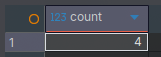
\includegraphics[width=0.425\textwidth]{pics/devices_count.png}
  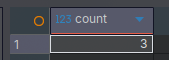
\includegraphics[width=0.425\textwidth]{pics/events_count.png}
  \caption*{Рисунок 1 - Вывод примера 1.}
\end{figure}

\subsection*{Пример 2: Статистика по идентификаторам устройств}

Запрос выводит сумму, минимум, максимум и среднее значение по столбцу \texttt{id} в таблице \texttt{devices}. Результат аналогичен представлению \texttt{device\_id\_stats}, но в одной строке.

\begin{minted}{sql}
select 
  sum(id) as sum_id,
  min(id) as min_id, 
  max(id) as max_id, 
  avg(id) as avg_id
from devices;
\end{minted}

\begin{figure}[H]
  \centering
  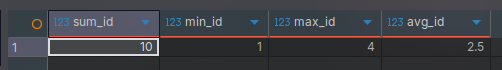
\includegraphics[width=0.95\textwidth]{pics/id_stats.png}
  \caption*{Рисунок 2 - Вывод примера 2.}
\end{figure}

\subsection*{Пример 3: Группировка событий по типу}

Запрос группирует события по их типу и подсчитывает количество событий каждого типа.

\begin{minted}{sql}
select event_type, count(*) as event_count
from events
group by event_type
order by event_count desc;
\end{minted}

\begin{figure}[H]
  \centering
  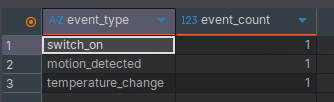
\includegraphics[width=0.6\textwidth]{pics/event_group.png}
  \caption*{Рисунок 3 - Вывод примера 3.}
\end{figure}

\subsection*{Пример 4: Фильтрация групп с помощью HAVING}

Запрос находит типы устройств, у которых подключено более одного устройства. Предложение \texttt{HAVING} фильтрует результаты после группировки.

\begin{minted}{sql}
select dt.type_name, count(d.id) as device_count
from devices d
join device_types dt on d.type_id = dt.id
group by dt.type_name
having count(d.id) > 1;
\end{minted}

\begin{figure}[H]
  \centering
  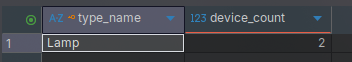
\includegraphics[width=0.6\textwidth]{pics/group_filter.png}
  \caption*{Рисунок 4 - Вывод примера 4.}
\end{figure}

\section*{Операторы, встроенные функции и работа с датами}

В PostgreSQL доступен широкий набор операторов и функций для обработки данных.

\subsection*{Пример 5: Логические операторы и сравнение с NULL}

Проверка логических выражений и корректное сравнение со значением \texttt{NULL}.

\begin{minted}{sql}
-- Логическое выражение
select not 1 < 2 and 3 < 4 or 5 = 5; -- true

-- Сравнение с NULL
select 1 is null or 5 is not null; -- true
\end{minted}

\begin{figure}[H]
  \centering
  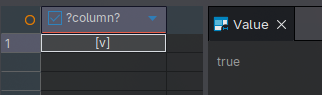
\includegraphics[width=0.425\textwidth]{pics/logic_1.png}
  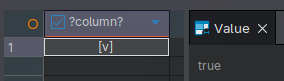
\includegraphics[width=0.425\textwidth]{pics/logic_2.png}
  \caption*{Рисунок 5 - Вывод примера 5.}
\end{figure}

\subsection*{Пример 6: Работа со строками}

Использование функций для конкатенации, изменения регистра и проверки по шаблону.

\begin{minted}{sql}
-- Конкатенация строк
select 'User: ' || username from users;

-- Приведение к нижнему регистру
select lower(email) from users;

-- Поиск по шаблону (пользователи с почтой на example.com)
select username from users where email like '%@example.com';
\end{minted}

\begin{figure}[H]
  \centering
  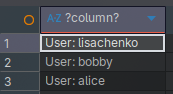
\includegraphics[width=0.31\textwidth]{pics/string_1.png}
  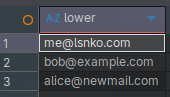
\includegraphics[width=0.31\textwidth]{pics/string_2.png}
  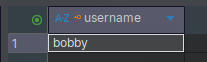
\includegraphics[width=0.31\textwidth]{pics/string_3.png}
  \caption*{Рисунок 6 - Вывод примера 6.}
\end{figure}

\subsection*{Пример 7: Работа с датами}

Примеры работы с типом данных \texttt{timestamp}, в частности со столбцом \texttt{created\_at} в таблице \texttt{events}.

\begin{minted}{sql}
-- Текущая дата и время
select now();

-- События за последние 24 часа (гипотетически)
select * from events 
where created_at > now() - interval '1 day';

-- Разница между датами (в днях)
select (now() - created_at) as age from events;
\end{minted}

\begin{figure}[H]
  \centering
  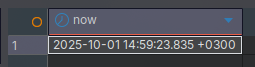
\includegraphics[width=0.425\textwidth]{pics/dates_1.png}\\
  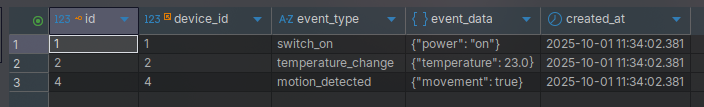
\includegraphics[width=0.95\textwidth]{pics/dates_2.png}\\
  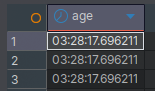
\includegraphics[width=0.425\textwidth]{pics/dates_3.png}
  \caption*{Рисунок 7 - Вывод примера 7.}
\end{figure}

\section*{Подзапросы и предложение WITH}

Подзапросы и общие табличные выражения (CTE) позволяют структурировать сложные запросы.

\subsection*{Пример 8: Простой подзапрос}

Запрос находит имена пользователей, которые владеют хабами с устройствами типа "Lamp".

\begin{minted}{sql}
select username 
from users 
where id in (
  select distinct h.user_id 
  from hubs h 
  join devices d on h.id = d.hub_id
  join device_types dt on d.type_id = dt.id
  where dt.type_name = 'Lamp'
);
\end{minted}

\begin{figure}[H]
  \centering
  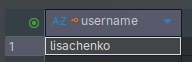
\includegraphics[width=0.425\textwidth]{pics/subquery.png}
  \caption*{Рисунок 8 - Вывод примера 8.}
\end{figure}

\subsection*{Пример 9: Использование WITH (CTE)}

Тот же запрос, переписанный с использованием CTE для улучшения читаемости.

\begin{minted}{sql}
with lamp_hubs as (
  select distinct h.user_id 
  from hubs h 
  join devices d on h.id = d.hub_id
  join device_types dt on d.type_id = dt.id
  where dt.type_name = 'Lamp'
)
select username 
from users 
where id in (select user_id from lamp_hubs);
\end{minted}

\begin{figure}[H]
  \centering
  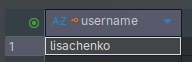
\includegraphics[width=0.425\textwidth]{pics/subquery.png}
  \caption*{Рисунок 9 - Вывод примера 9.}
\end{figure}

% \clearpage
\section*{RETURNING}

\texttt{RETURNING} позволяет получить данные об изменённых или вставленных строках в одном запросе.

\subsection*{Пример 10: Вставка с RETURNING}

Добавление нового типа устройства и получение его идентификатора.

\begin{minted}{sql}
insert into device_types(type_name) 
values ('Smart Socket') 
returning id;
\end{minted}

\begin{figure}[H]
  \centering
  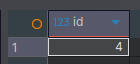
\includegraphics[width=0.425\textwidth]{pics/returning.png}
  \caption*{Рисунок 10 - Вывод примера 10.}
\end{figure}

\subsection*{Пример 11: Обновление с RETURNING}

Обновление статуса устройства и возврат его нового состояния.

\begin{minted}{sql}
update devices 
set status = '{"power": "off", "brightness": 50}' 
where name = 'Ceiling Lamp' 
returning *;
\end{minted}

\begin{figure}[H]
  \centering
  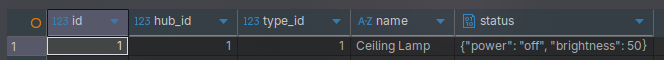
\includegraphics[width=0.95\textwidth]{pics/returning_2.png}
  \caption*{Рисунок 11 - Вывод примера 11.}
\end{figure}

\section*{Анализ плана выполнения запросов (EXPLAIN)}

Для оптимизации производительности используется команда \texttt{EXPLAIN}.

\subsection*{Пример 12: Последовательное сканирование}

План запроса на выборку всех устройств. Так как в условии нет фильтрации по индексу, используется последовательное сканирование (Sequential Scan).

\begin{minted}{sql}
explain (analyze, buffers) select * from devices;
\end{minted}

\begin{figure}[H]
  \centering
  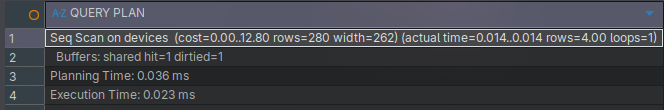
\includegraphics[width=0.95\textwidth]{pics/explain_1.png}
  \caption*{Рисунок 12 - Вывод примера 12.}
\end{figure}

\subsection*{Пример 13: Индексное сканирование}

План запроса на выборку устройства по его уникальному идентификатору. Здесь используется индексное сканирование (Index Scan), так как столбец \texttt{id} является первичным ключом и имеет индекс.

\begin{minted}{sql}
explain (analyze, buffers) select * from devices where id = 1;
\end{minted}

\begin{figure}[H]
  \centering
  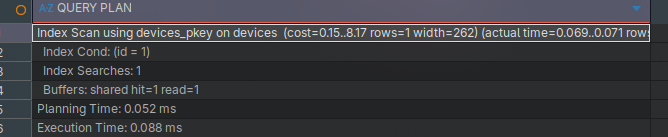
\includegraphics[width=0.95\textwidth]{pics/explain_2.png}
  \caption*{Рисунок 13 - Вывод примера 13.}
\end{figure}

\subsection*{Пример 14: Соединение таблиц}

План запроса для представления \texttt{device\_full\_info}, которое соединяет несколько таблиц. PostgreSQL может выбрать различные стратегии соединения (Nested Loop, Hash Join, Merge Join) в зависимости от статистики и настроек.

\begin{minted}{sql}
explain (analyze, format json) 
select * from device_full_info;
\end{minted}

\begin{figure}[H]
  \centering
  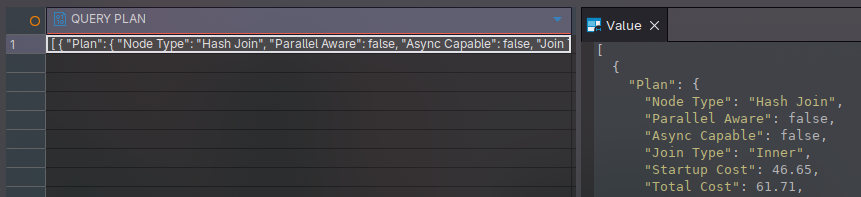
\includegraphics[width=0.95\textwidth]{pics/join.png}
  \caption*{Рисунок 14 - Вывод примера 14.}
\end{figure}

\begin{minted}{json}
[
  {
    "Plan": {
      "Node Type": "Hash Join",
      "Parallel Aware": false,
      "Async Capable": false,
      "Join Type": "Inner",
      "Startup Cost": 46.65,
      "Total Cost": 61.71,
      "Plan Rows": 280,
      "Plan Width": 676,
      "Actual Startup Time": 0.100,
      "Actual Total Time": 0.104,
      "Actual Rows": 4.00,
      "Actual Loops": 1,
      "Disabled": false,
      "Inner Unique": true,
      "Hash Cond": "(h.user_id = u.id)",
      "Shared Hit Blocks": 4,
      "Shared Read Blocks": 0,
      "Shared Dirtied Blocks": 1,
      "Shared Written Blocks": 0,
      "Local Hit Blocks": 0,
      "Local Read Blocks": 0,
      "Local Dirtied Blocks": 0,
      "Local Written Blocks": 0,
      "Temp Read Blocks": 0,
      "Temp Written Blocks": 0,
      "Plans": [
        {
          "Node Type": "Hash Join",
          "Parent Relationship": "Outer",
          "Parallel Aware": false,
          "Async Capable": false,
          "Join Type": "Inner",
          "Startup Cost": 34.62,
          "Total Cost": 48.92,
          "Plan Rows": 280,
          "Plan Width": 562,
          "Actual Startup Time": 0.077,
          "Actual Total Time": 0.080,
          "Actual Rows": 4.00,
          "Actual Loops": 1,
          "Disabled": false,
          "Inner Unique": true,
          "Hash Cond": "(d.hub_id = h.id)",
          "Shared Hit Blocks": 3,
          "Shared Read Blocks": 0,
          "Shared Dirtied Blocks": 1,
          "Shared Written Blocks": 0,
          "Local Hit Blocks": 0,
          "Local Read Blocks": 0,
          "Local Dirtied Blocks": 0,
          "Local Written Blocks": 0,
          "Temp Read Blocks": 0,
          "Temp Written Blocks": 0,
          "Plans": [
            { ...
\end{minted}

\subsection*{Пример 15: Анализ плана соединения четырёх таблиц}

Запрос из Примера 10 соединяет четыре таблицы. PostgreSQL может выбрать разные стратегии соединения. Рассмотрим их.

\subsubsection*{По умолчанию (обычно Hash Join или Nested Loop)}
\begin{minted}{sql}
explain (analyze, buffers)
select e.id, u.username
from events e
join devices d on e.device_id = d.id
join hubs h on d.hub_id = h.id
join users u on h.user_id = u.id;
\end{minted}

\begin{figure}[H]
  \centering
  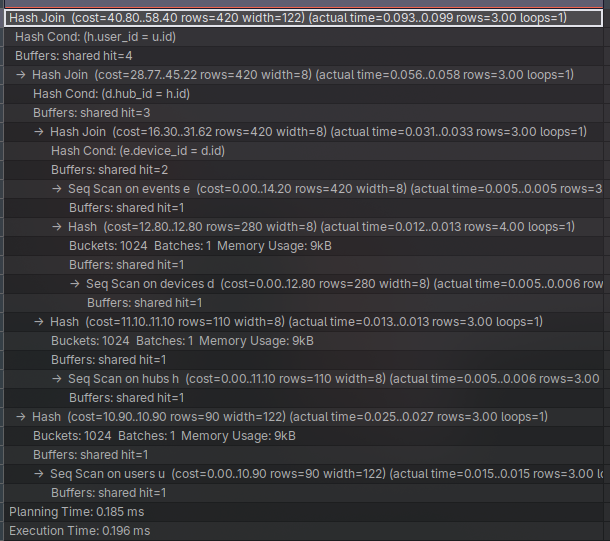
\includegraphics[width=0.75\textwidth]{pics/hash_join.png}
  \caption*{Рисунок 15.1 - Вывод примера 15 с Hash Join.}
\end{figure}

\subsubsection*{Принудительное использование Nested Loop}
\begin{minted}{sql}
set enable_hashjoin = off;
set enable_mergejoin = off;
explain (analyze, buffers)
select e.id, u.username
from events e
join devices d on e.device_id = d.id
join hubs h on d.hub_id = h.id
join users u on h.user_id = u.id;
-- reset
set enable_hashjoin = on;
set enable_mergejoin = on;
\end{minted}

\begin{figure}[H]
  \centering
  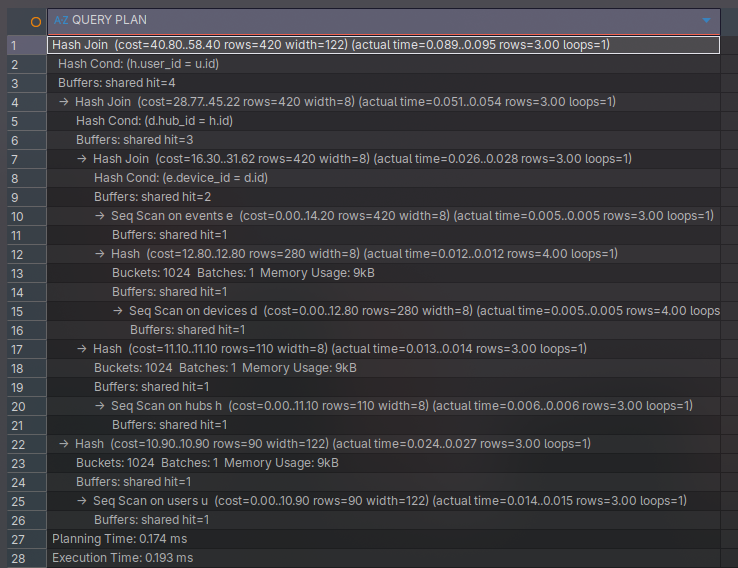
\includegraphics[width=0.75\textwidth]{pics/nested_loop.png}
  \caption*{Рисунок 15.2 - Вывод примера 15 с Nested Loop.}
\end{figure}

\clearpage
\subsubsection*{Принудительное использование Merge Join}
\begin{minted}{sql}
set enable_hashjoin = off;
set enable_nestloop = off;
explain (analyze, buffers)
select e.id, u.username
from events e
join devices d on e.device_id = d.id
join hubs h on d.hub_id = h.id
join users u on h.user_id = u.id;
-- reset
set enable_hashjoin = on;
set enable_nestloop = on;
\end{minted}

\begin{figure}[H]
  \centering
  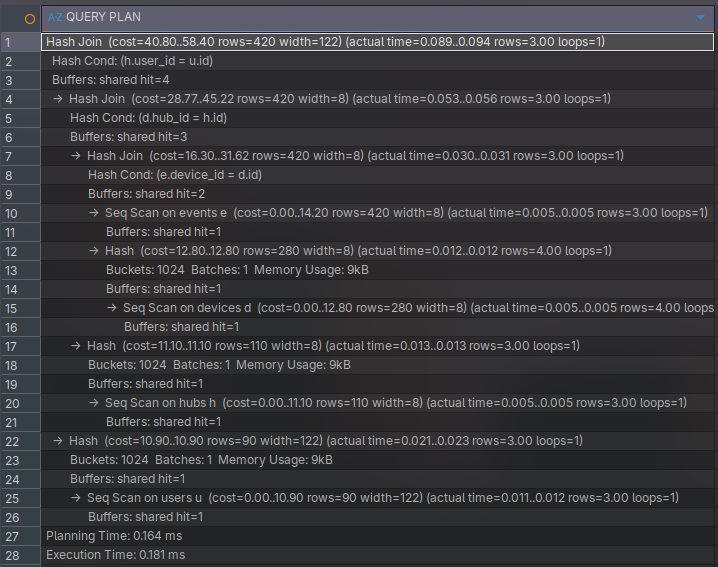
\includegraphics[width=0.75\textwidth]{pics/merge_join.png}
  \caption*{Рисунок 15.3 - Вывод примера c Merge Join.}
\end{figure}

\clearpage
\section*{Вывод}

В ходе выполнения лабораторной работы №2\_2 были освоены ключевые аспекты языка DML в PostgreSQL. Были изучены и применены на практике агрегатные функции (\texttt{count}, \texttt{sum}, \texttt{avg}, \texttt{min}, \texttt{max}) и предложение \texttt{HAVING} для фильтрации сгруппированных данных. Продемонстрировано использование различных операторов, встроенных функций для работы со строками и датами. Рассмотрены механизмы подзапросов и общих табличных выражений (\texttt{WITH}) для повышения читаемости сложных запросов. Также изучено предложение \texttt{RETURNING} для получения информации об изменённых строках. Наконец, с помощью команды \texttt{EXPLAIN} был проведен анализ планов выполнения запросов, включая сравнение различных стратегий соединения (Nested Loop, Hash Join, Merge Join) для запросов с участием нескольких таблиц, что является важным инструментом для оптимизации производительности базы данных.
\newpage

\setminted{style = rainbow_dash, fontsize = \small} % https://pygments.org/styles/  

\section*{Приложение А1. Исходный код}
\inputminted{Dockerfile}{../Containerfile}

\section*{Приложение А2. SQL-скрипты}

\subsection*{Агрегатные функции и HAVING}
\begin{minted}{sql}
-- Пример 1
select count(*) from devices;
select count(*) from events;

-- Пример 2
select 
  sum(id) as sum_id,
  min(id) as min_id, 
  max(id) as max_id, 
  avg(id) as avg_id
from devices;

-- Пример 3
select event_type, count(*) as event_count
from events
group by event_type
order by event_count desc;

-- Пример 4
select dt.type_name, count(d.id) as device_count
from devices d
join device_types dt on d.type_id = dt.id
group by dt.type_name
having count(d.id) > 1;
\end{minted}

\subsection*{Операторы и функции}
\begin{minted}{sql}
-- Пример 5
select not 1 < 2 and 3 < 4 or 5 = 5;
select 1 is null or 5 is not null;

-- Пример 6
select 'User: ' || username from users;
select lower(email) from users;
select username from users where email like '%@example.com';

-- Пример 7
select now();
select * from events where created_at > now() - interval '1 day';
select (now() - created_at) as age from events;
\end{minted}

\subsection*{Подзапросы и WITH}
\begin{minted}{sql}
-- Пример 8
select username 
from users 
where id in (
  select distinct h.user_id 
  from hubs h 
  join devices d on h.id = d.hub_id
  join device_types dt on d.type_id = dt.id
  where dt.type_name = 'Lamp'
);

-- Пример 9
with lamp_hubs as (
  select distinct h.user_id 
  from hubs h 
  join devices d on h.id = d.hub_id
  join device_types dt on d.type_id = dt.id
  where dt.type_name = 'Lamp'
)
select username 
from users 
where id in (select user_id from lamp_hubs);
\end{minted}

\subsection*{RETURNING и EXPLAIN}
\begin{minted}{sql}
-- Пример 11
insert into device_types(type_name) values ('Smart Socket') returning id;

-- Пример 12
update devices set status = '{"power": "off", "brightness": 50}' where name = 'Ceiling Lamp' returning *;

-- Пример 13
explain (analyze, buffers) select * from devices;

-- Пример 14
explain (analyze, buffers) select * from devices where id = 1;

-- Пример 15 — Nested Loop
set enable_hashjoin = off; set enable_mergejoin = off;
explain (analyze, buffers) select e.id, u.username from events e join devices d on e.device_id = d.id join hubs h on d.hub_id = h.id join users u on h.user_id = u.id;
set enable_hashjoin = on; set enable_mergejoin = on;

-- Пример 15 — Merge Join
set enable_hashjoin = off; set enable_nestloop = off;
explain (analyze, buffers) select e.id, u.username from events e join devices d on e.device_id = d.id join hubs h on d.hub_id = h.id join users u on h.user_id = u.id;
set enable_hashjoin = on; set enable_nestloop = on;
\end{minted}

\end{document}